ระบบระบุตัวตนของบุคคล\textsuperscript{\cite{luo2019alignedreid++}}\textsuperscript{\cite{zhang2017alignedreid}} คือการระบุตัวตนของบุคคลภายในวิดีโอหรือระหว่างสองภาพ สามารถนำมาประยุกต์ใช้ในด้านของการรักษาความปลอดภัย 
หรือการตามหาบุคคล ซึ่งการระบุตัวตนของบุคคลนั้นเป็นปัญหาที่ท้าทาย เนื่องจากคุณลักษณะทั่วไปของบุคคลในภาพไม่เพียงพอต่อการระบุตัวตนภายในภาพว่าเป็นบุคคลคนเดียวกันได้ ซึ่งวิธีการที่ใช้ในการระบุตัวตนของบุคคลเรียกว่า 
Dynamically Matching Local Information (DMLI) ที่สามารถจัดแนวรายละเอียดข้อมูลของภาพและเพิ่มประสิทธิภาพให้สูงขึ้น 
ถึงแม้ว่า DMLI นั้นจะไม่ใช่วิธีการที่มีประสิทธิภาพสูงสุดแต่มีประสิทธิภาพใกล้เคียงกับโมเดลอื่นๆ แต่ผู้วิจัยสามารถนำวิธีนี้มาประยุกต์เข้ากับงานวิจัยครั้งนี้ได้สะดวกที่สุด จึงนำวิธีการนี้มาใช้สำหรับงานวิจัยครั้งนี้

\begin{figure}[!ht]
	\centering
	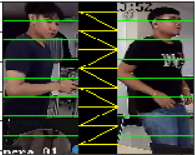
\includegraphics[width=0.3\textwidth]{chapter2/images/alignedreid.png}
		\caption{การแบ่งภาพออกเป็น 8 ส่วนของระบบระบุตัวตนของบุคคล}
    	\label{fig:alignedreid}
\end{figure}

การทำงานของระบบระบุตัวตนของบุคคลจะเริ่มจากการแบ่งภาพออกเป็น 8 ส่วนและนำคุณลักษณะทั่วไปของภาพมาผ่านกระบวนการ normalization เพื่อลดความซ้ำซ้อนของข้อมูล 
แล้วนำมาเปรียบเทียบความแตกต่างของคุณลักษณะทั่วไปของภาพโดยใช้วิธี euclidean distance หลังจากนั้นใช้วิธี DMLI หาความแตกต่างออกมา โดยค่าที่ได้ออกมาจะเรียกว่า aligned distance ถ้าค่าที่ออกมาใกล้เคียงกับศูนย์
จะหมายถึงบุคคลในภาพทั้งสองเป็นบุคคลเดียวกัน โดยใช้การกำหนดเกณฑ์ของ aligned distance สำหรับระบุตัวตนของบุคคลในภาพว่าเป็นบุคคลเดียวกันหรือไม่

โดยชุดข้อมูลที่นำมาใช้สำหรับการทำโมเดลปัญญาประดิษฐ์ได้แก่
\begin{enumerate}
	\item{Market1501 เป็นชุดข้อมูลที่เก็บข้อมูลภาพของบุคคลโดยใช้กล้องจำนวนหกตัว ถ่ายภาพบุคคลที่ด้านหน้าของซุปเปอร์มาร์เก็ตในมหาวิทยาลัย Tsinghua}
	\item{DukeMTMCReID เป็นชุดข้อมูลที่เก็บข้อมูลภาพของบุคคลโดยใช้กล้องจำนวนแปดตัว ถ่ายภาพบุคคลที่วิทยาเขตของมหาวิทยาลัย Duke ซึ่งมีการเก็บภาพมากถึงสองล้านภาพของนักศึกษาสองพันคน }
	\item{CUHK-03 เป็นชุดข้อมูลที่เก็บภาพของบุคคลที่มหาวิทยาลัยที่ฮ่องกง}
	\item{MSMT17 เป็นชุดข้อมูลที่เก็บข้อมูลภาพของบุคคลโดยใช้กล้องจำนวนสิบห้าตัว โดยที่กล้องแต่ละตัวจะไม่ได้ตั้งอยู่สถานที่เดียวกัน และเก็บข้อมูลที่ในวันที่มีสภาพอากาศต่างกัน}
\end{enumerate}

โดยทุกชุดข้อมูลจะใช้โครงสร้าง (architecture) ResNet50 ในการสร้างโมเดลปัญญาประดิษฐ์ และทดสอบด้วยวิธี Global+DMLI คือการนำคุณลักษณะทั่วไปและคุณลักษณะจำเพาะของภาพที่ได้มาจากโมเดลปัญญาประดิษฐ์ นำมาหาค่าระยะความแตกต่าง โดยที่ค่าระยะความแตกต่างของคุณลักษณะทั่วไปสามาหาได้โดยใช้วิธี Euclidean distance และค่าระยะความแตกต่างของคุณลักษณะจำเพาะสามารถหาได้โดยใช้วิธี DMLI และนำมาเทียบกับชุดข้อมูลทดสอบเพื่อคำนวณหาค่า rank1 และ mAP โดยที่ค่า rank1 หมายถึงค่าอัตราร้อยละของความมั่นใจสูงสุดของโมเดลปัญญาประดิษฐ์ที่ทำนายออกมาถูกต้อง 
และค่า mAP คือการหาค่าเฉลี่ยความแม่นยำในแต่ละหมวดหมู่ ซึ่งสามารถดูค่า rank1 และ mAP ของโมเดลปัญญาประดิษฐ์สำหรับการทำระบุตัวตนของบุคคลได้ในหัวข้อที่ \ref{sec:reid_ex}

วิธีการคำนวณของ DMLI ในขั้นตอนการสร้างโมเดลปัญญาประดิษฐ์ของการระบุตัวตนบุคคล
\begin{equation}
d_{i,j} = \frac{e^{\left \| f_{i} - g_{j} \right \|^{2}} - 1}{e^{\left \| f_{i} - g_{j} \right \|^{2}} + 1} \qquad i,j \epsilon 1,2,3,..H
\end{equation}

โดยที่
\begin{conditions}
d		&		เมทริกซ์ของระยะความแตกต่างที่น้อยที่สุดของคุณลักษณะจำเพาะของทั้งสองภาพ			\\
f		&		ค่าคุณลักษณะจำเพาะของรูปภาพที่ 1				\\
g		&		ค่าคุณลักษณะจำเพาะของรูปภาพที่ 2				\\
H		&		จำนวนภาพแนวตั่งที่แบ่งออกมา
\end{conditions}

\begin{equation}
S_{i,j} = \begin{cases}
d_{i,j} & \text{ if } i=1,j=1 \\ 
S_{i-1,j}+d_{i,j} & \text{ if } i\neq 1,j=1 \\ 
S_{i,j-1}+d_{i,j} & \text{ if } i=1,j\neq1 \\ 
min(S_{i-1,j},S_{i,j-1}) & \text{ if } i\neq1,j\neq1 
\end{cases}
\end{equation}

เมื่อทำการคำนวณ $S_{i,j}$ ซึ่งเป็นผลรวมของระยะความแตกต่างที่น้อยที่สุดแล้วตัวสุดท้ายของ $S_{i,j}$ จะเป็นระยะความแตกต่างที่น้อยที่สุดที่ของคุณลักษณะจำเพาะของทั้งสองภาพ แต่ในกรณีที่ทางผู้วิจัยนำมาใช้งานค่า $d_{i,j}$ นั้นจะเป็นค่าที่ได้มาจากการนำคุณลักษณะทั่วไปของภาพมาทำ euclidean distance แทน
